\chapter{Технологическая часть}

В данной части рассматриваются описываются выбранные средства реализации, структура классов программы, а также приводятся листинги реализации алгоритмов и приводится демонстрационный пример интерфейса программы.

\section{Средства реализации}
Для написания курсового проекта был выбран язык $C\#$ версии 7.3~\cite{CSharp}, предоставляющий достаточный набор инструментов для реализации спроектированного ПО. В частности, язык поддерживает объектно-ориентированную модель разработки, что позволяет выделять отдельные сущности задачи в виде классов.

В качестве интегрированной среды разработки была выбрана Microsoft Visual Studio 2022~\cite{VS2022}, предоставляющая достаточный функционал для написания, профилирования и отладки написанной программы, равно как и реализация пользовательского графического интерфейса ПО.

\section{Структура программы}
На рисунке~\ref{fig:SceneObjects} представлена диаграмма разработанных классов.
\clearpage
\begin{figure}[H]
	\centering
	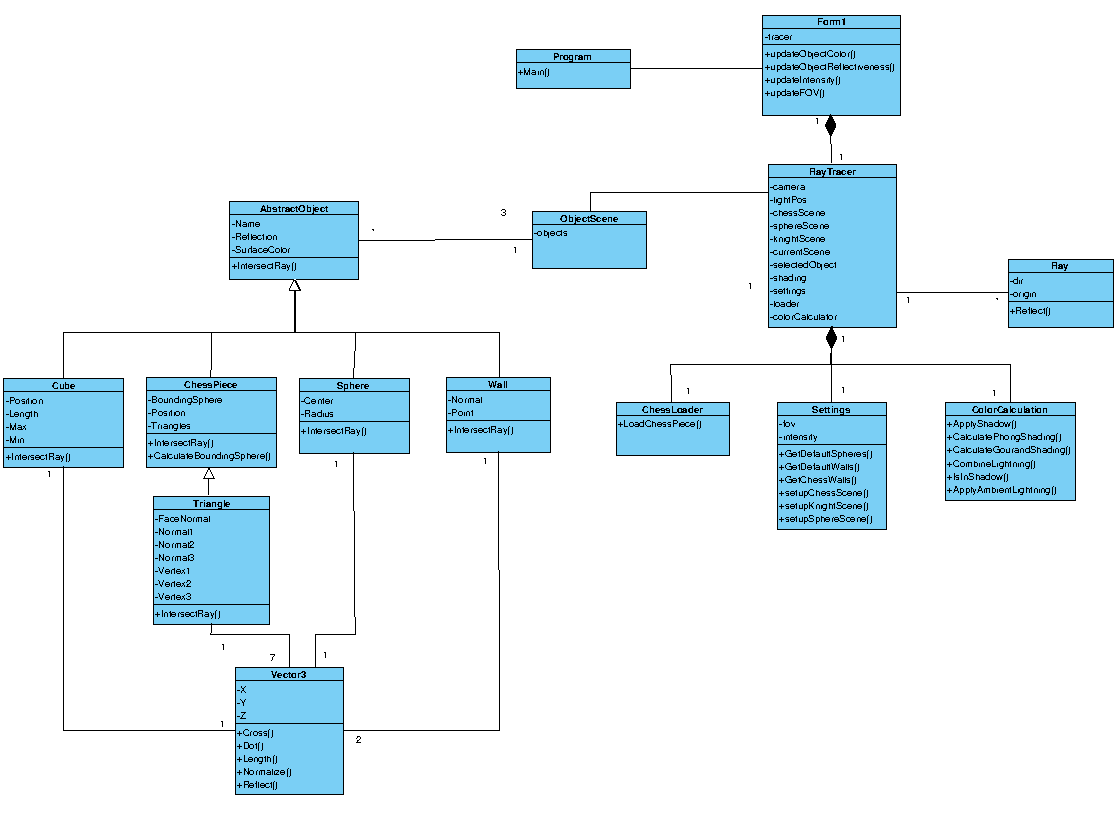
\includegraphics[width=\textwidth]{Class_Diagram_UML}
	\caption{Диаграмма классов объектов сцены}
	\label{fig:SceneObjects}
\end{figure}

Разработанная программа состоит из следующих классов:
\begin{enumerate}
	\item структурные классы программы
	\begin{itemize}
		\item Program -- точка входа в программу;
		\item Form1 -- класс, представляющий графический интерфейс программы;
	\end{itemize}
	\item базовые математические классы
	\begin{itemize}
		\item Ray -- класс луча трассировки, также используется для представления камеры в программе;
		\item Vector3 -- класс трехмерного вектора, поддерживающий математические операции над векторами;
	\end{itemize}
	\item классы объектов сцены
	\begin{itemize}
		\item AbstractObject -- абстрактный класс, определяющий общий для всех объектов интерфейс;
		\item Cube -- класс, представляющий куб в качестве объекта сцены;
		\item ChessPiece -- класс, представляющий шахматную фигуру в качестве объекта сцены;
		\item Triangle -- класс для представления треугольных полигонов, из которых состоят шахматные фигуры;
		\item Sphere -- класс, представляющий сферу в качестве объекта сцены;
		\item Wall -- класс, представляющий стену в качестве объекта сцены;
	\end{itemize}
	\item ObjectScene -- класс, представляющий сцену объектов. Содержит список всех объектов сцены.
	\item вспомогательные классы
	\begin{itemize}
		\item ChessLoader -- класс, предназначенный для загрузки моделей шахматных фигур из объектных файлов;
		\item Settings -- класс с настройками для трассировки лучей;
		\item ColorCalculation -- класс, реализующий логику реализации выбранной модели освещения;
	\end{itemize}
	\item RayTracer -- класс, реализующий основную логику приложения.
\end{enumerate}

\section{Реализация алгоритмов}
В соответствии со схемой, изображенной на рисунке~\ref{fig:RayTracing} был реализован алгоритм трассировки лучей, приведенный на листинге~\ref{lst:RayTracing}.

\clearpage
\begin{center}
	\begin{lstlisting}[linewidth=\linewidth, label={lst:RayTracing}, captionpos={t}, caption={Алгоритм трассировки лучей}]
	private Color TraceRay(Ray ray, ObjectScene scene, Vector3 lightPos, Color backgroundColor, int depth)
	{
		if (depth <= 0)
			return backgroundColor;
		
		double closestDistance = double.MaxValue;
		Vector3 hitNormal = new Vector3(0, 0, 0);
		AbstractObject closestObject = null;
		
		foreach (var obj in scene.objects)
		{
			if (obj.IntersectRay(ray, out double dist, out Vector3 normal) && dist < closestDistance)
			{
				closestDistance = dist;
				hitNormal = normal;
				closestObject = obj;
			}
		}
		
		if (closestObject == null)
			return backgroundColor;
		
		Vector3 hitPoint = ray.origin + ray.dir * closestDistance;
		Color objectColor = ((dynamic)closestObject).SurfaceColor;
		Color lightingColor = CalculateLighting(hitPoint, hitNormal, lightPos, objectColor, scene);
		
		if (closestObject.Reflection > 0)
		{
			Vector3 reflectionDir = ray.dir.Reflect(hitNormal);
			Color reflectionColor = TraceRay(new Ray(hitPoint, reflectionDir), scene, lightPos, backgroundColor, depth - 1);
			lightingColor = MixColors(lightingColor, reflectionColor, closestObject.Reflection);
		}
		return lightingColor;
	}
	\end{lstlisting}
\end{center}

На листингах~\ref{lst:SphereIntersection}~-~\ref{lst:ChessIntersection},~\ref{lst:CubeIntersection} приведены алгоритмы пересечения объектов сцены с лучом.

\begin{center}
	\begin{lstlisting}[linewidth=\linewidth, label={lst:SphereIntersection}, captionpos={t}, caption={Алгоритм поиска точки пересечения луча со сферой}]
		public override bool IntersectRay(Ray ray, out double t, out Vector3 Normal)
		{
			Vector3 oc = ray.origin - Center;
			double a = ray.dir.Dot(ray.dir);
			double b = 2.0 * oc.Dot(ray.dir);
			double c = oc.Dot(oc) - Radius * Radius;
			double discriminant = b * b - 4 * a * c;
			Normal = null;
			
			if (discriminant < 0)
			{
				t = 0;
				return false;
			}
			
			t = (-b - Math.Sqrt(discriminant)) / (2.0 * a);
			
			if (t > 0)
			Normal = (ray.origin + ray.dir * t - Center).Normalize();
			
			return t > 0;
		}
	\end{lstlisting}
\end{center}

\clearpage
\begin{center}
	\begin{lstlisting}[linewidth=\linewidth, label={lst:WallIntersection}, captionpos={t}, caption={Алгоритм поиска точки пересечения луча с плоскостью (стеной)}]
		public override bool IntersectRay(Ray ray, out double t, out Vector3 normal)
		{
			t = 0;
			normal = new Vector3(0, 0, 0);
			
			double denom = Normal.Dot(ray.dir);
			if (Math.Abs(denom) > 1e-6)
			{
				t = (Point - ray.origin).Dot(Normal) / denom;
				if (t >= 0)
				{
					normal = Normal;
					return true;
				}
			}
			return false;
		}
	\end{lstlisting}
\end{center}

Реализация алгоритма пересечения луча трассировки с кубом представлена в листинге~\ref{lst:CubeIntersection} (см. приложение Б).

\clearpage
\begin{center}
	\begin{lstlisting}[linewidth=\linewidth, label={lst:TriangleIntersection}, captionpos={t}, caption={Алгоритм поиска точки пересечения луча с треугольным полигоном}]
		public bool IntersectRay(Ray ray, out double distance, out Vector3 barycentricCoords)
		{
			barycentricCoords = new Vector3(0, 0, 0);
			distance = 0;
			Vector3 edge1 = Vertex2 - Vertex1;
			Vector3 edge2 = Vertex3 - Vertex1;
			Vector3 pvec = ray.dir.Cross(edge2);
			double det = edge1.Dot(pvec);
			const double epsilon = 1e-8;
			if (Math.Abs(det) < epsilon)
			return false;
			
			double invDet = 1.0 / det;
			
			Vector3 tvec = ray.origin - Vertex1;
			double u = tvec.Dot(pvec) * invDet;
			
			if (u < 0.0 || u > 1.0)
			return false;
			
			Vector3 qvec = tvec.Cross(edge1);
			double v = ray.dir.Dot(qvec) * invDet;
			
			if (v < 0.0 || u + v > 1.0)
			return false;
			
			distance = edge2.Dot(qvec) * invDet;
			
			if (distance > epsilon)
			{
				barycentricCoords = new Vector3(1 - u - v, u, v);
				return true;
			}
			
			return false;
		}
	\end{lstlisting}
\end{center}


\clearpage
\begin{center}
	\begin{lstlisting}[linewidth=\linewidth, label={lst:ChessIntersection}, captionpos={t}, caption={Алгоритм поиска точки пересечения луча с шахматной фигурой}]
		public override bool IntersectRay(Ray ray, out double distance, out Vector3 interpolatedNormal)
		{
			distance = double.MaxValue;
			interpolatedNormal = new Vector3(0, 0, 0);
			
			if (!BoundingSphere.IntersectRay(ray, out double sphereDist, out Vector3 Normal))
			{
				return false;
			}
			
			bool hit = false;
			foreach (var triangle in Triangles)
			{
				if (triangle.IntersectRay(ray, out double dist, out Vector3 barycentricCoords) && dist < distance)
				{
					distance = dist;
					hit = true;
					
					interpolatedNormal =
					barycentricCoords.X * triangle.Normal1 +
					barycentricCoords.Y * triangle.Normal2 +
					barycentricCoords.Z * triangle.Normal3;
					
					interpolatedNormal = interpolatedNormal.Normalize();
				}
			}
			
			return hit;
		}
	\end{lstlisting}
\end{center}

\section{Функциональное тестирование}
В таблице \ref{tab:func} приведены функциональные тесты для программы, визуализирующей трехмерные сцены объектов. Все тесты пройдены программой успешно.

	
\begin{longtable}{|r|c|c|c|}
	\caption{\label{tab:func}Функциональные тесты (начало)} \\ \hline
	№ & \makecell{Состояние программы \\ до теста} & Изменяемый параметр/событие & Ожидаемый результат \\ \hline
	\endfirsthead
	\caption[]{Функциональные тесты (окончание табл. \ref{tab:func})} \\ \hline
	№ & \makecell{Состояние программы \\ до теста} & Изменяемый параметр/событие & Ожидаемый результат \\ \hline
	\endhead
	\hline
	\endfoot
	\hline
	\endlastfoot
	
	1 & --- & \makecell{Нажатие кнопки\\<<Визуализировать>>} & \makecell{Визуализация сцены с \\двумя сферами и первой\\камерой} \\ \hline
	2 & --- & \makecell{Выбор сцены \\<<Сцена с шахматными \\фигурами>>;\\Нажатие кнопки\\<<Визуализировать>>} & \makecell{Визуализация сцены с \\шахматными фигурами и\\ первой камерой} \\ \hline
	3 & --- & \makecell{Выбор сцены \\<<Сцена с конем и сферой>>;\\Нажатие кнопки\\<<Визуализировать>>} & \makecell{Визуализация сцены с \\конем, кубом и сферой} \\ \hline
	4 & \makecell{Выбрана и\\визуализирована\\сцена с двумя сферами} & \makecell{Выбор камеры №2\\Нажатие кнопки\\<<Визуализировать>>} & \makecell{Визуализация сцены с \\двумя сферами и второй\\камерой} \\ \hline
	5 & \makecell{Выбрана и\\визуализирована\\сцена с двумя сферами} & \makecell{Выбор камеры №3\\Нажатие кнопки\\<<Визуализировать>>} & \makecell{Визуализация сцены с \\двумя сферами и третьей\\камерой} \\ \hline
	6 & \makecell{Выбрана и \\визуализирована сцена \\с шахматными фигурами\\и первой камерой} & \makecell{Выбор камеры №2\\Нажатие кнопки\\<<Визуализировать>>} & \makecell{Визуализация сцены с \\с шахматными фигурами\\и второй камерой} \\ \hline
	7 & \makecell{Выбрана и \\визуализирована \\сцена с двумя сферами и \\третьей камерой} & \makecell{Изменение поля зрения\\на 90 градусов\\Нажатие кнопки\\<<Визуализировать>>} & \makecell{Визуализация сцены с \\двумя сферами и третьей\\камерой с углом\\обзора 90 градусов} \\ \hline
	8 & \makecell{Выбрана и \\визуализирована \\сцена с конем и сферой\\и третьей камерой} & \makecell{Выбор фигуры коня нажатием\\левой кнопки мыши;\\Изменение цвета коня на\\ желтый; Нажатие кнопки\\<<Визуализировать>>} & \makecell{Визуализация сцены с \\желтым конем и сферой\\с третьей камерой} \\ \hline
	9 & \makecell{Выбрана и \\визуализирована \\сцена с конем и сферой\\и второй камерой} & \makecell{Выбор куба в \\списке объектов;\\Изменение зеркальности\\куба на 95\%;\\Нажатие кнопки\\<<Визуализировать>>} & \makecell{Визуализация сцены с \\конем, зеркальным кубом\\ и сферой со второй\\камерой} \\ \hline
	10 & \makecell{Выбрана и \\визуализирована \\сцена с двумя сферами\\и первой камерой} & \makecell{Увеличение интенсивности \\света до 80\%;\\Нажатие кнопки\\<<Визуализировать>>} & \makecell{Визуализация сцены с \\двумя сферами с первой\\камерой и с \\интенсивностью\\ освещения 80\% \\от максимальной} \\ \hline
	11 & \makecell{Выбрана и \\визуализирована \\сцена с двумя сферами\\и второй камерой} & \makecell{Включение сглаживания;\\Изменение числа лучей на 64;\\Нажатие кнопки\\<<Визуализировать>>} & \makecell{Визуализация сцены с \\двумя сферами со второй\\камерой и со сглаживаем} \\ \hline
	12 & \makecell{Выбрана и \\визуализирована сцена с \\конем, кубом и сферой\\ с первой камерой} & \makecell{Включение глубины поля;\\Изменение расстояния до\\фокальной точки на 4;\\Нажатие кнопки\\<<Визуализировать>>} & \makecell{Визуализация сцены с \\конем, кубом и сферой\\ с первой камерой и с \\эффектом глубины поля} \\ \hline
	13 & \makecell{Выбрана и \\визуализирована \\сцена с двумя сферами\\и первой камерой} & \makecell{Изменение глянцевости\\поверхностей на 0\% и \\ зеркальности на 0\%;\\Нажатие кнопки\\<<Визуализировать>>} & \makecell{Визуализация сцены с \\двумя сферами с первой\\камерой с матовым\\ эффектом} \\ \hline
	14 & \makecell{Выбрана и \\визуализирована \\сцена с двумя сферами\\и первой камерой} & \makecell{Изменение глянцевости\\поверхностей на 100\% и\\ зеркальности на 20\%;\\Нажатие кнопки\\<<Визуализировать>>} & \makecell{Визуализация сцены с \\двумя сферами с первой\\камерой с глянцевым\\ эффектом} \\ \hline
\end{longtable}

На рисунках~\ref{fig:test1}~-~\ref{fig:test14} представлены визуализации тестов из таблицы~\ref{tab:func}.
\begin{figure}[H]
	\centering
	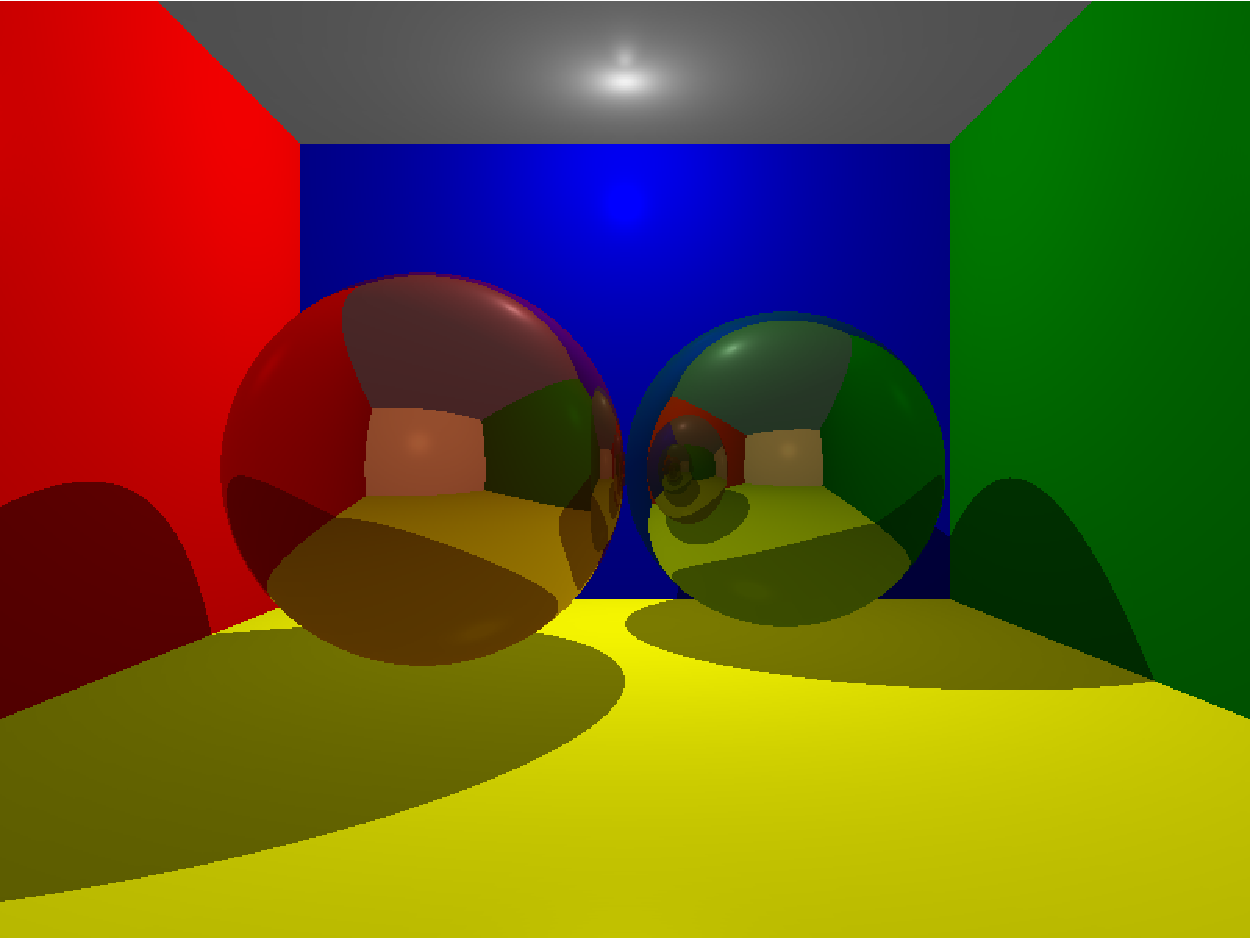
\includegraphics[width=0.55\textwidth]{test1}
	\caption{Визуализация функционального теста №1}
	\label{fig:test1}
\end{figure}
\begin{figure}[H]
	\centering
	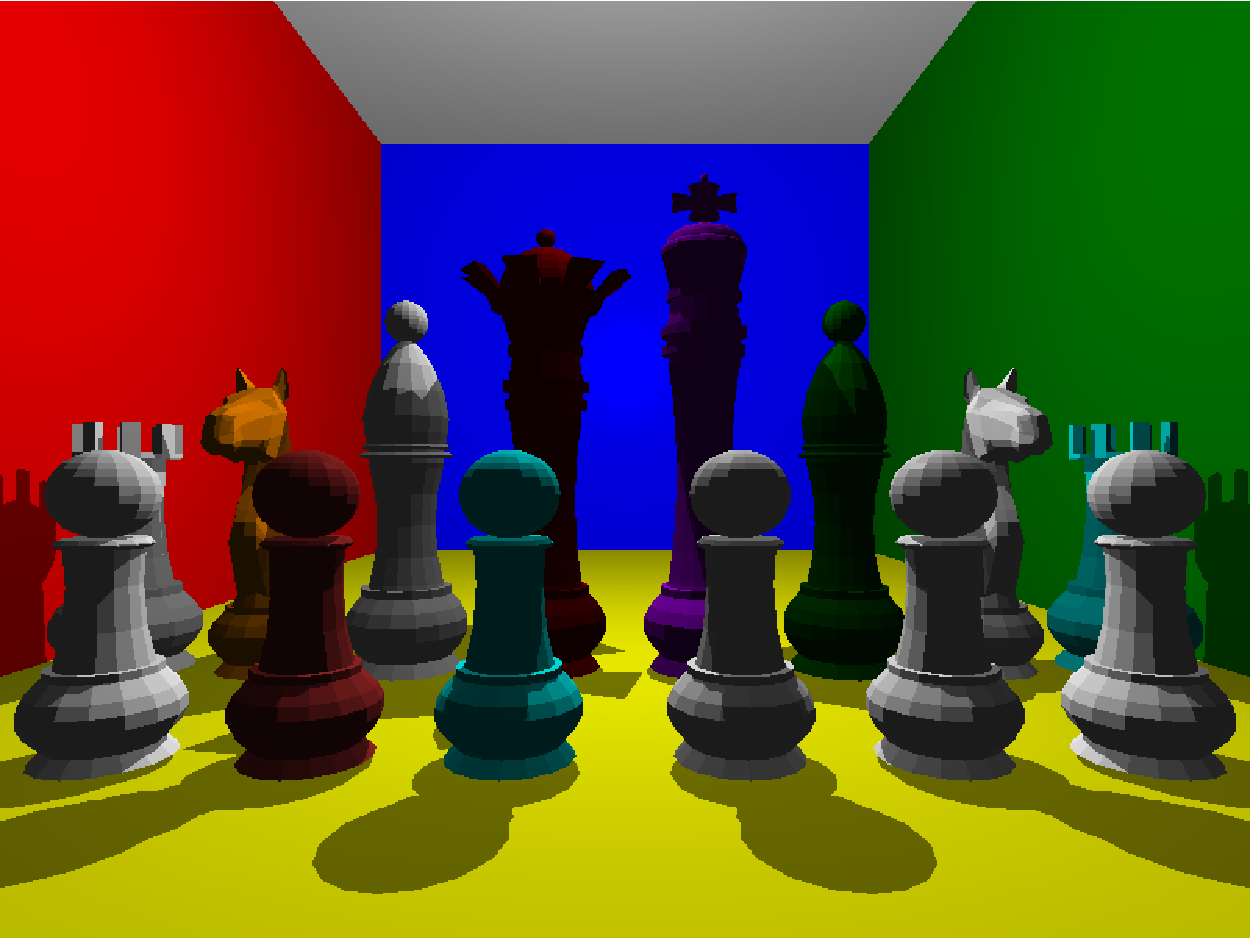
\includegraphics[width=0.55\textwidth]{test2}
	\caption{Визуализация функционального теста №2}
	\label{fig:test2}
\end{figure}
\begin{figure}[H]
	\centering
	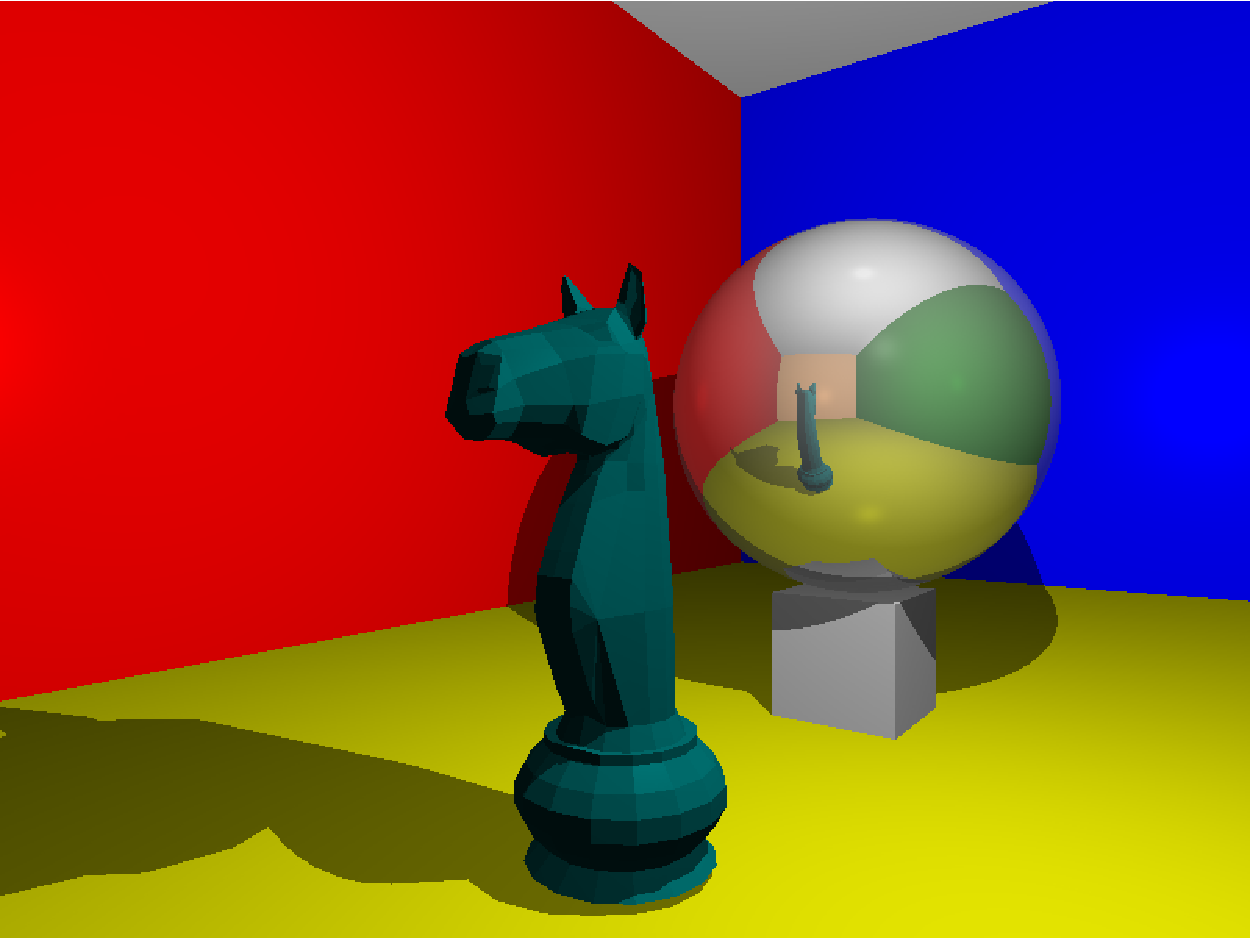
\includegraphics[width=0.55\textwidth]{test3}
	\caption{Визуализация функционального теста №3}
	\label{fig:test3}
\end{figure}

\begin{figure}[H]
	\centering
	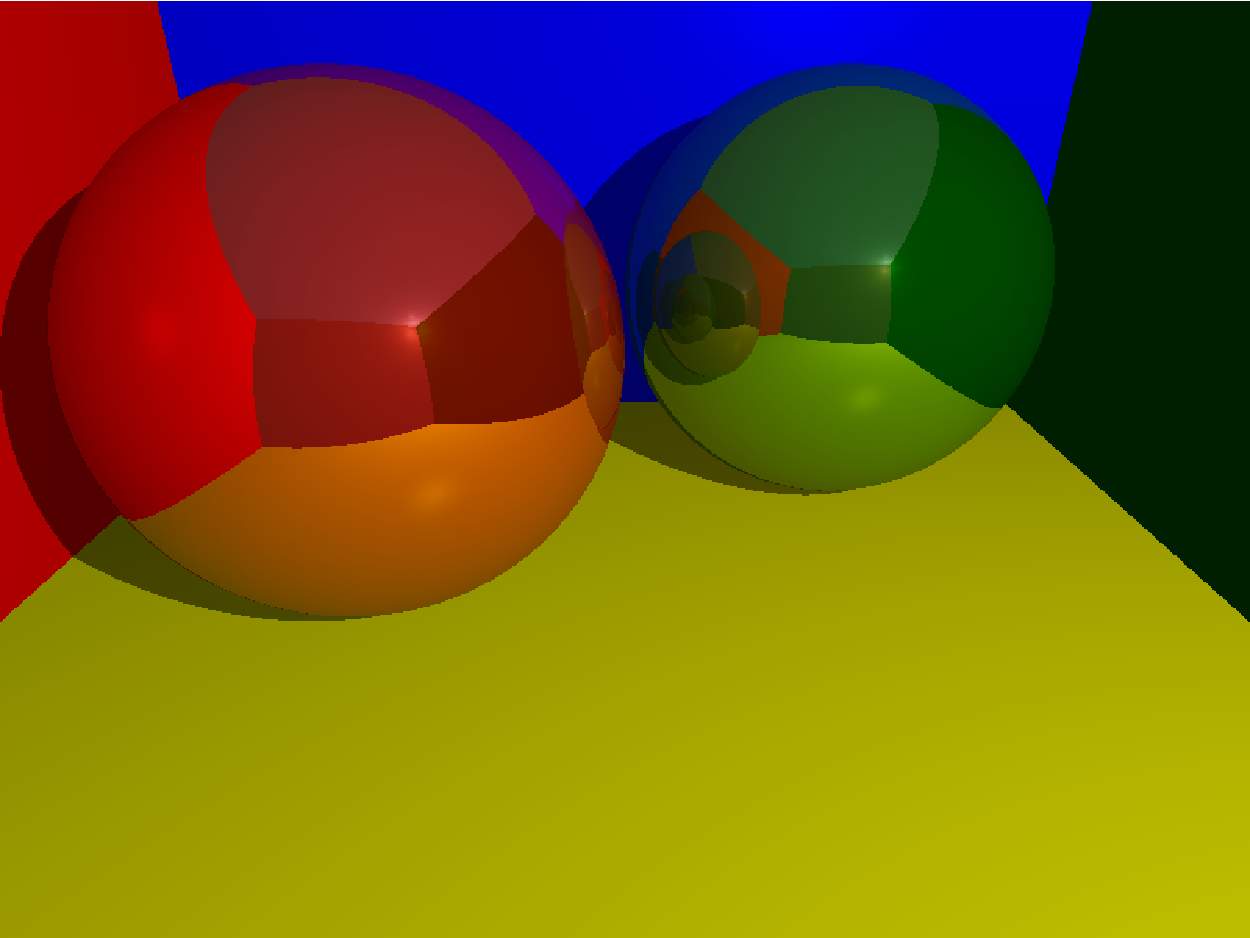
\includegraphics[width=0.55\textwidth]{test4}
	\caption{Визуализация функционального теста №4}
	\label{fig:test4}
\end{figure}
\begin{figure}[H]
	\centering
	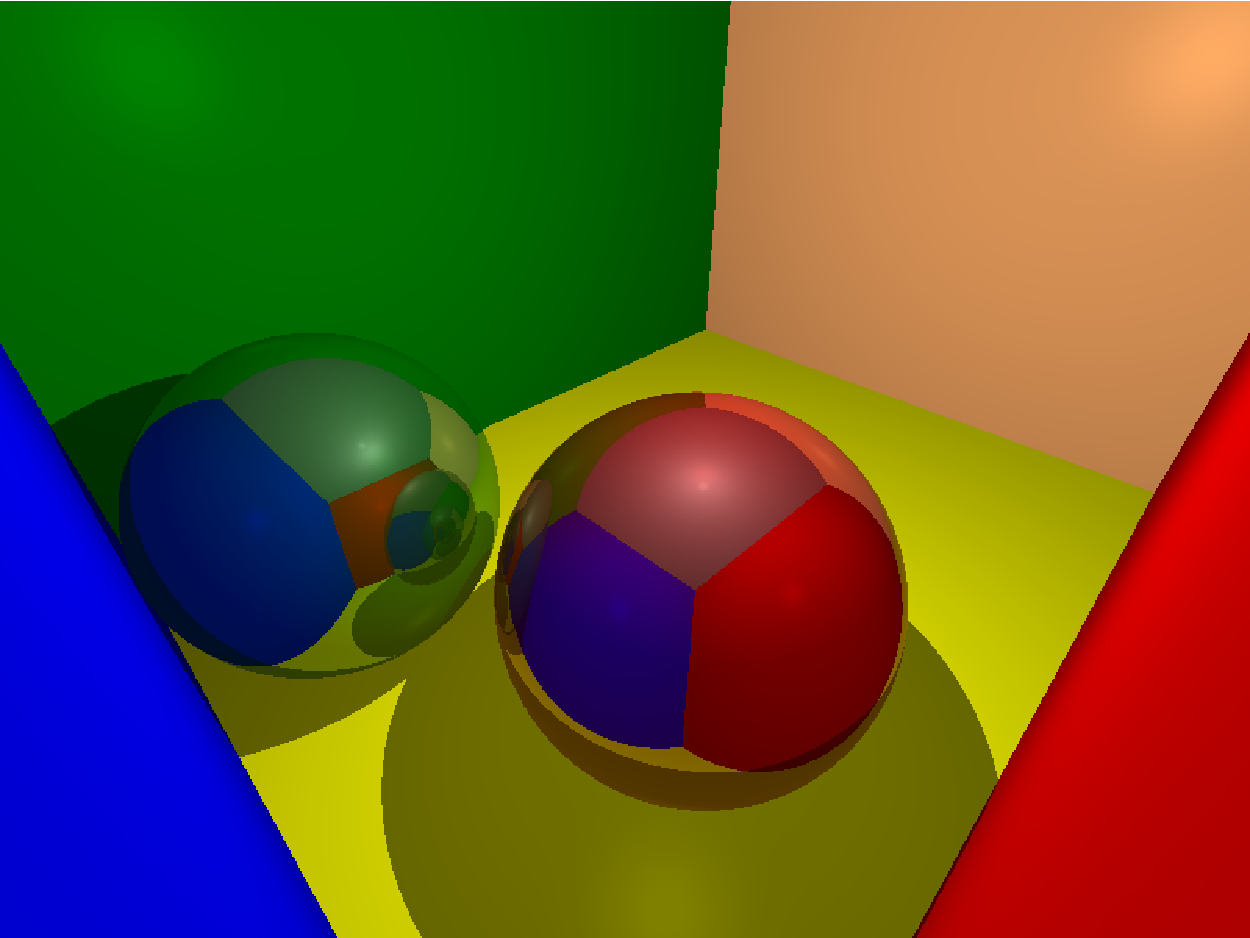
\includegraphics[width=0.55\textwidth]{test5}
	\caption{Визуализация функционального теста №5}
	\label{fig:test5}
\end{figure}
\begin{figure}[H]
	\centering
	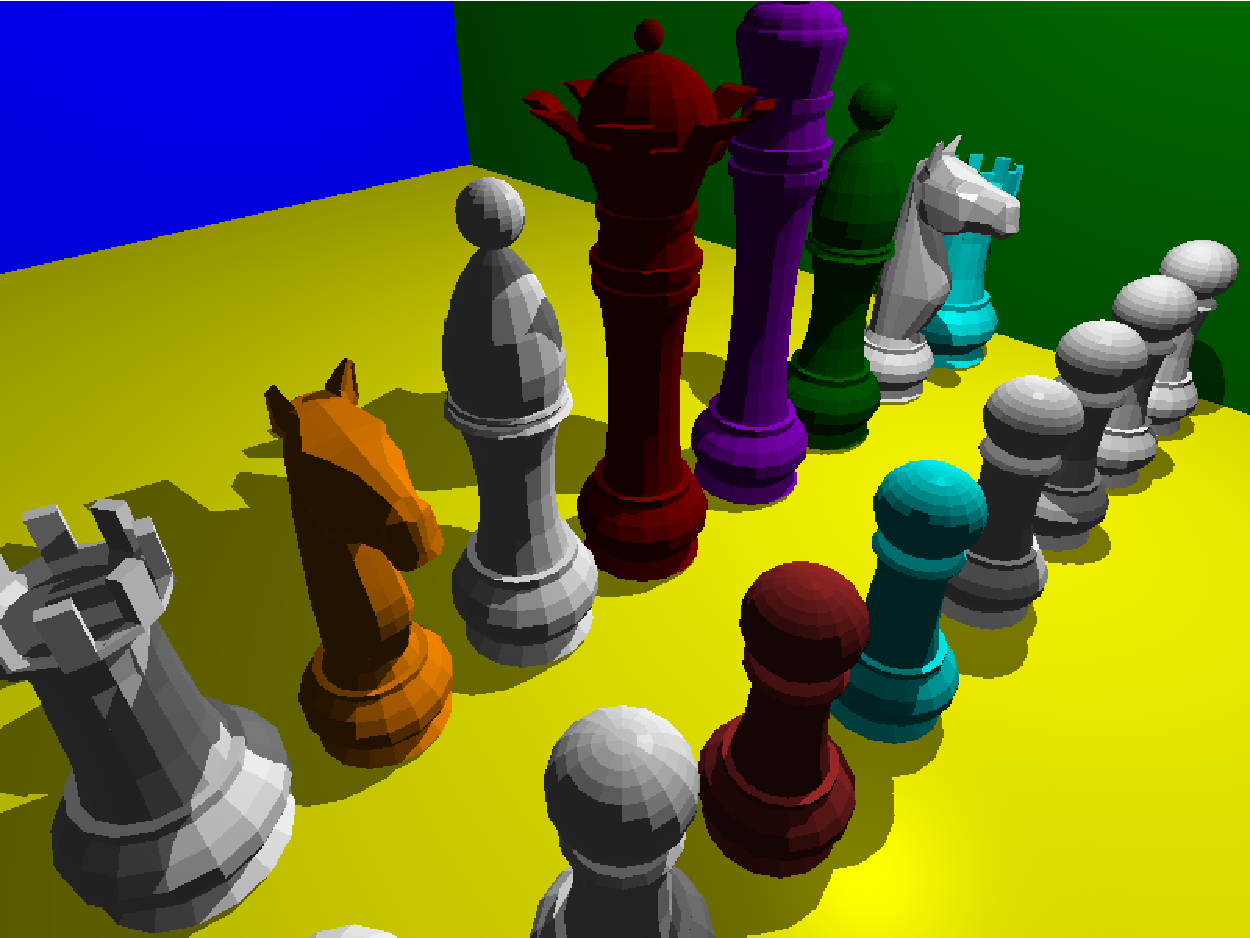
\includegraphics[width=0.55\textwidth]{test6}
	\caption{Визуализация функционального теста №6}
	\label{fig:test6}
\end{figure}

\begin{figure}[H]
	\centering
	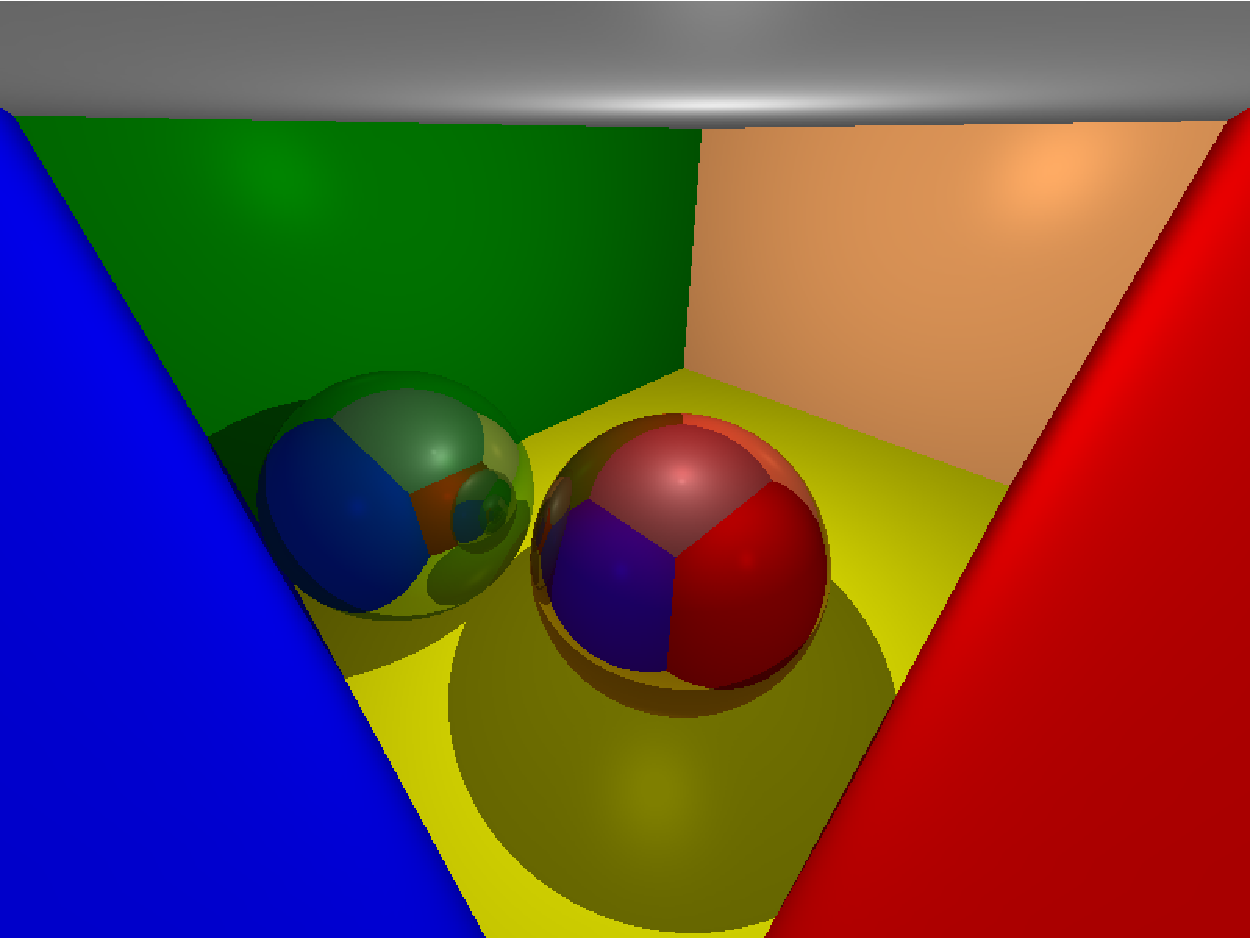
\includegraphics[width=0.55\textwidth]{test7}
	\caption{Визуализация функционального теста №7}
	\label{fig:test7}
\end{figure}
\begin{figure}[H]
	\centering
	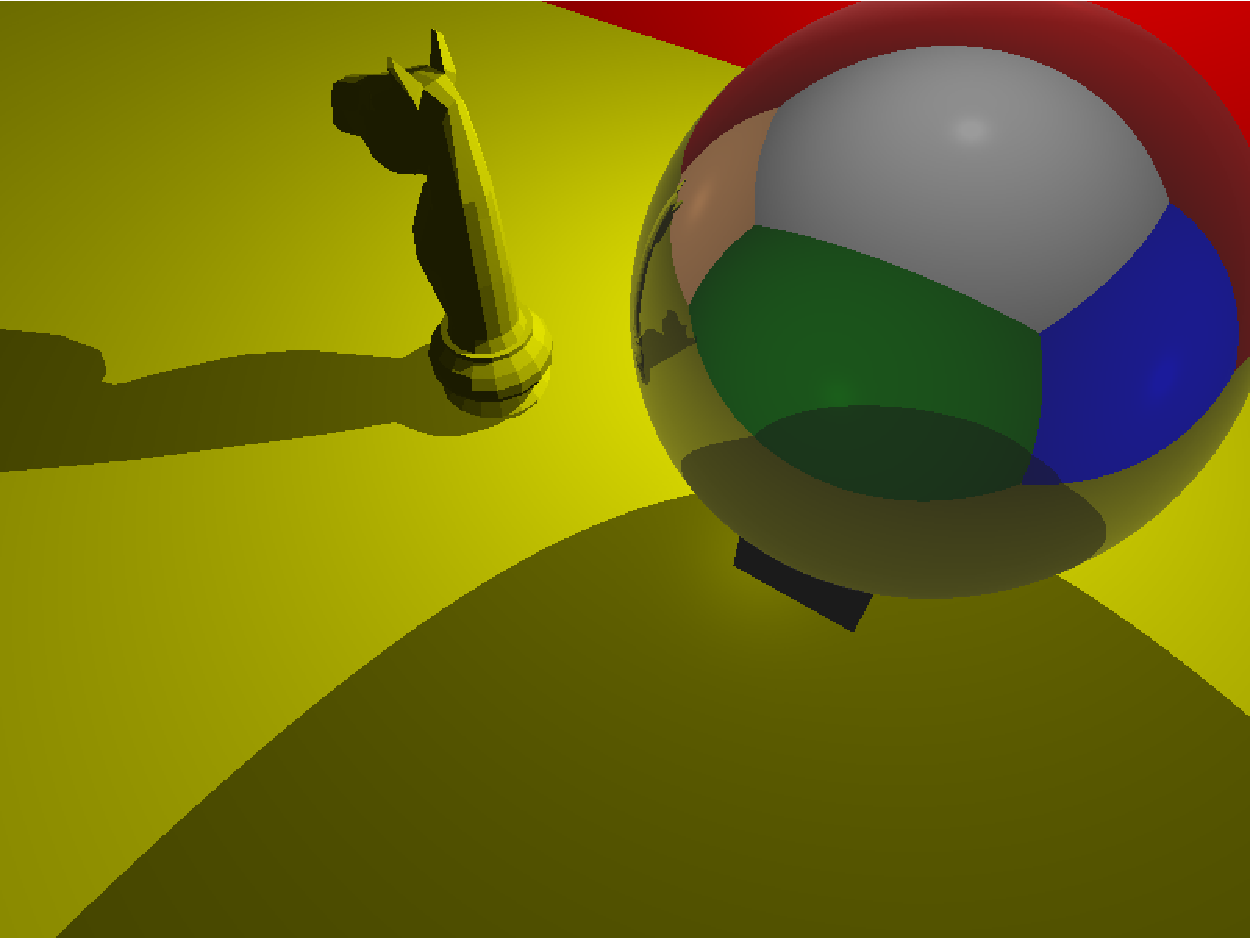
\includegraphics[width=0.55\textwidth]{test8}
	\caption{Визуализация функционального теста №8}
	\label{fig:test8}
\end{figure}
\begin{figure}[H]
	\centering
	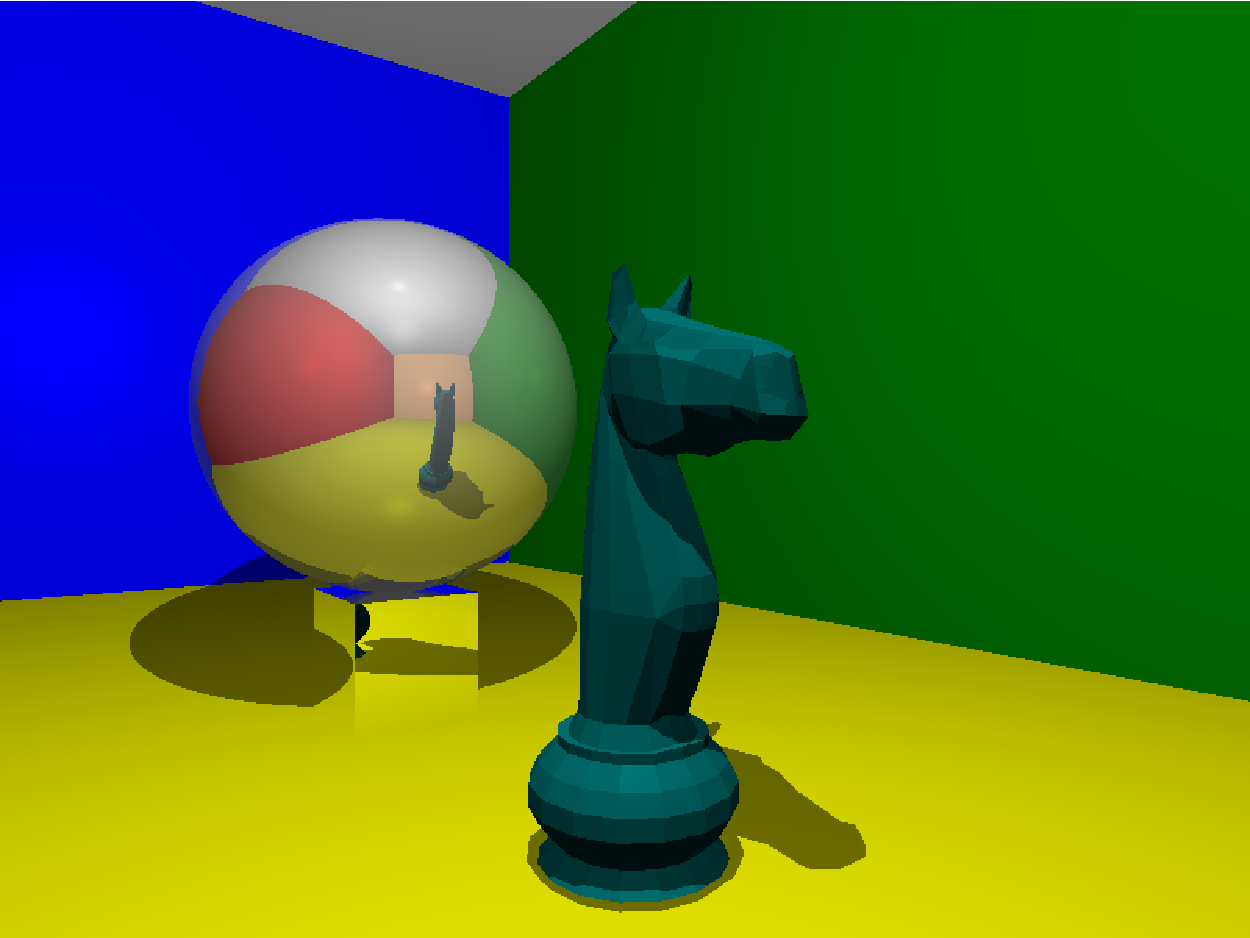
\includegraphics[width=0.55\textwidth]{test9}
	\caption{Визуализация функционального теста №9}
	\label{fig:test9}
\end{figure}

\begin{figure}[H]
	\centering
	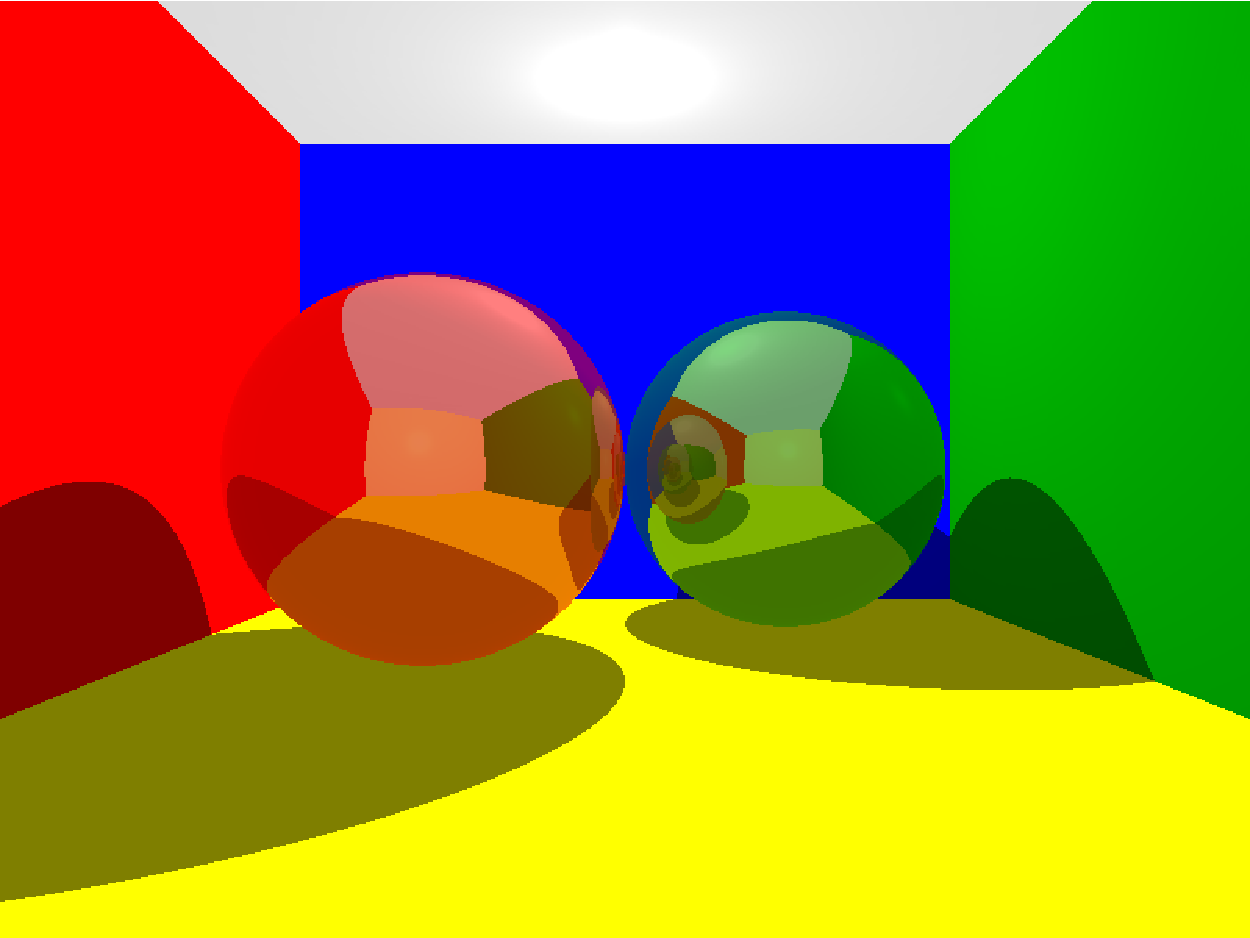
\includegraphics[width=0.55\textwidth]{test10}
	\caption{Визуализация функционального теста №10}
	\label{fig:test10}
\end{figure}
\begin{figure}[H]
	\centering
	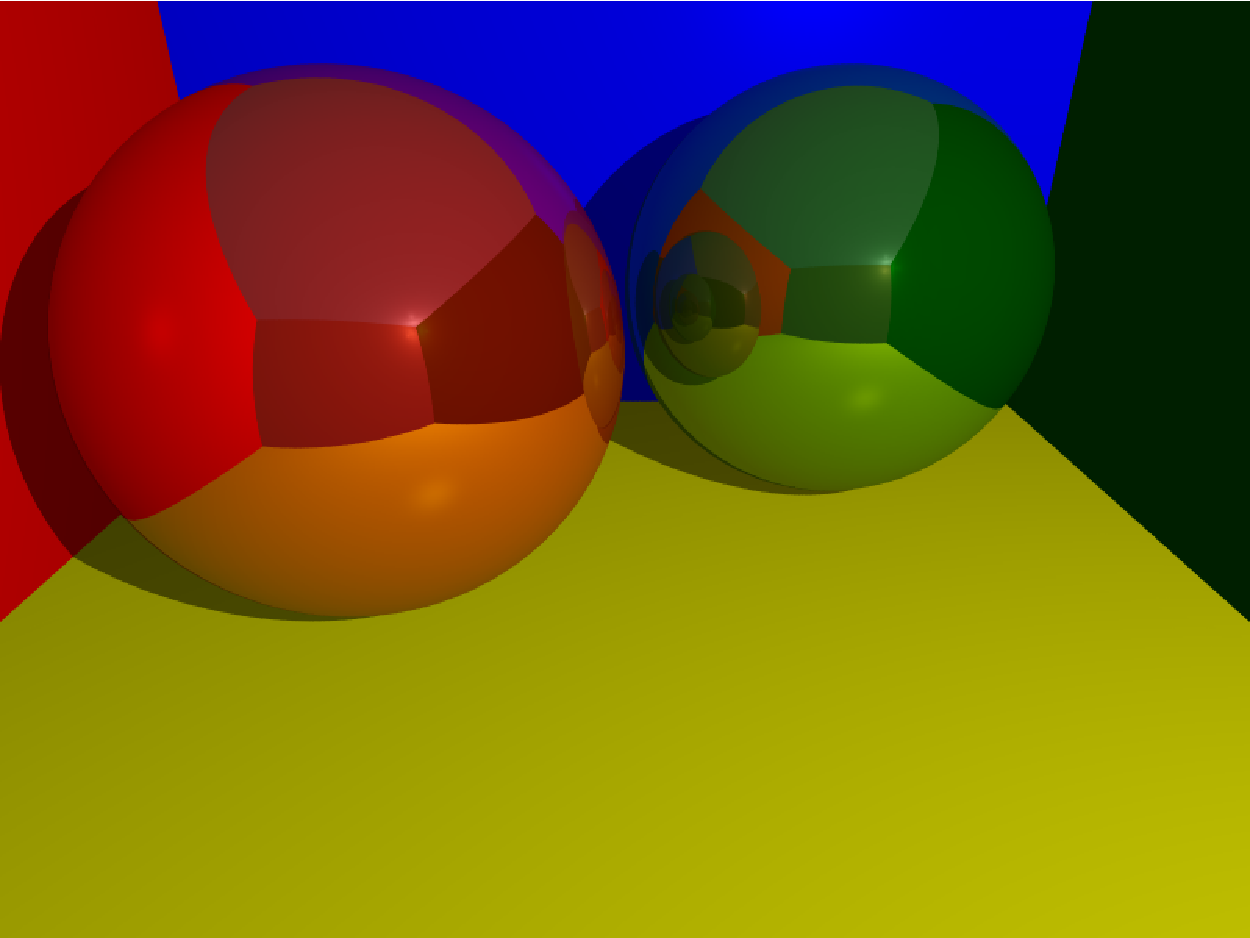
\includegraphics[width=0.55\textwidth]{test11}
	\caption{Визуализация функционального теста №11}
	\label{fig:test11}
\end{figure}
\begin{figure}[H]
	\centering
	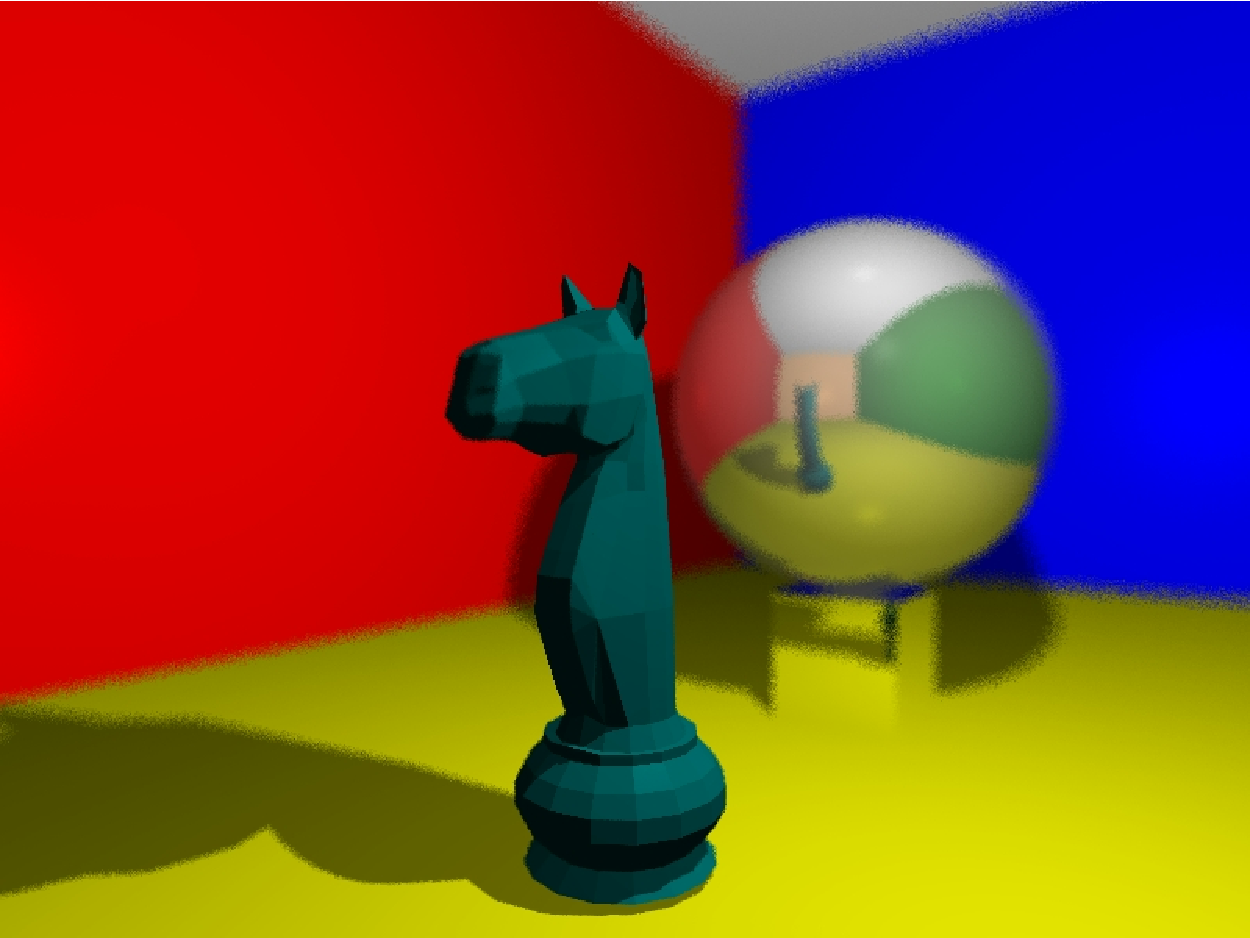
\includegraphics[width=0.55\textwidth]{test12}
	\caption{Визуализация функционального теста №12}
	\label{fig:test12}
\end{figure}
\begin{figure}[H]
	\centering
	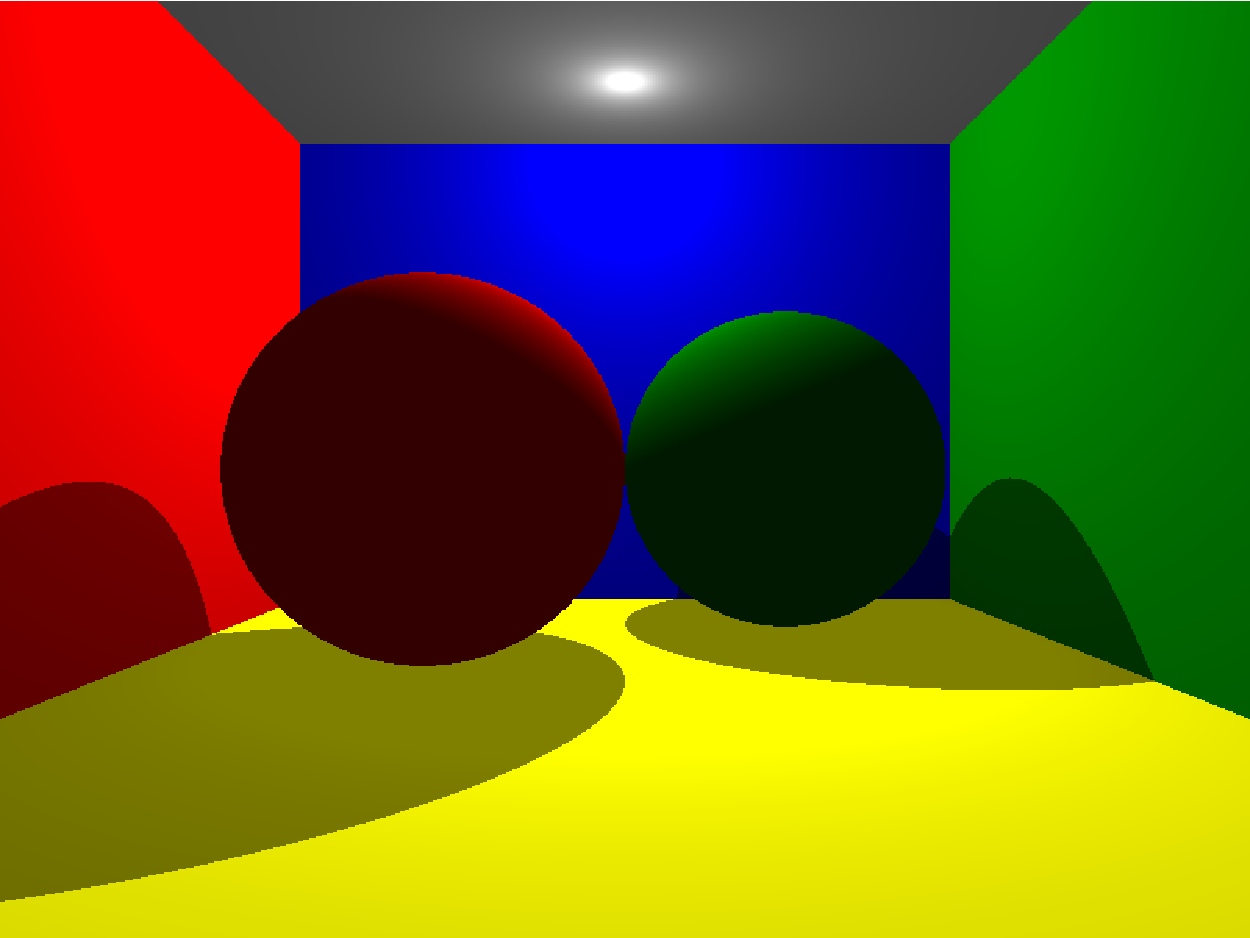
\includegraphics[width=0.55\textwidth]{test13}
	\caption{Визуализация функционального теста №13}
	\label{fig:test13}
\end{figure}
\begin{figure}[H]
	\centering
	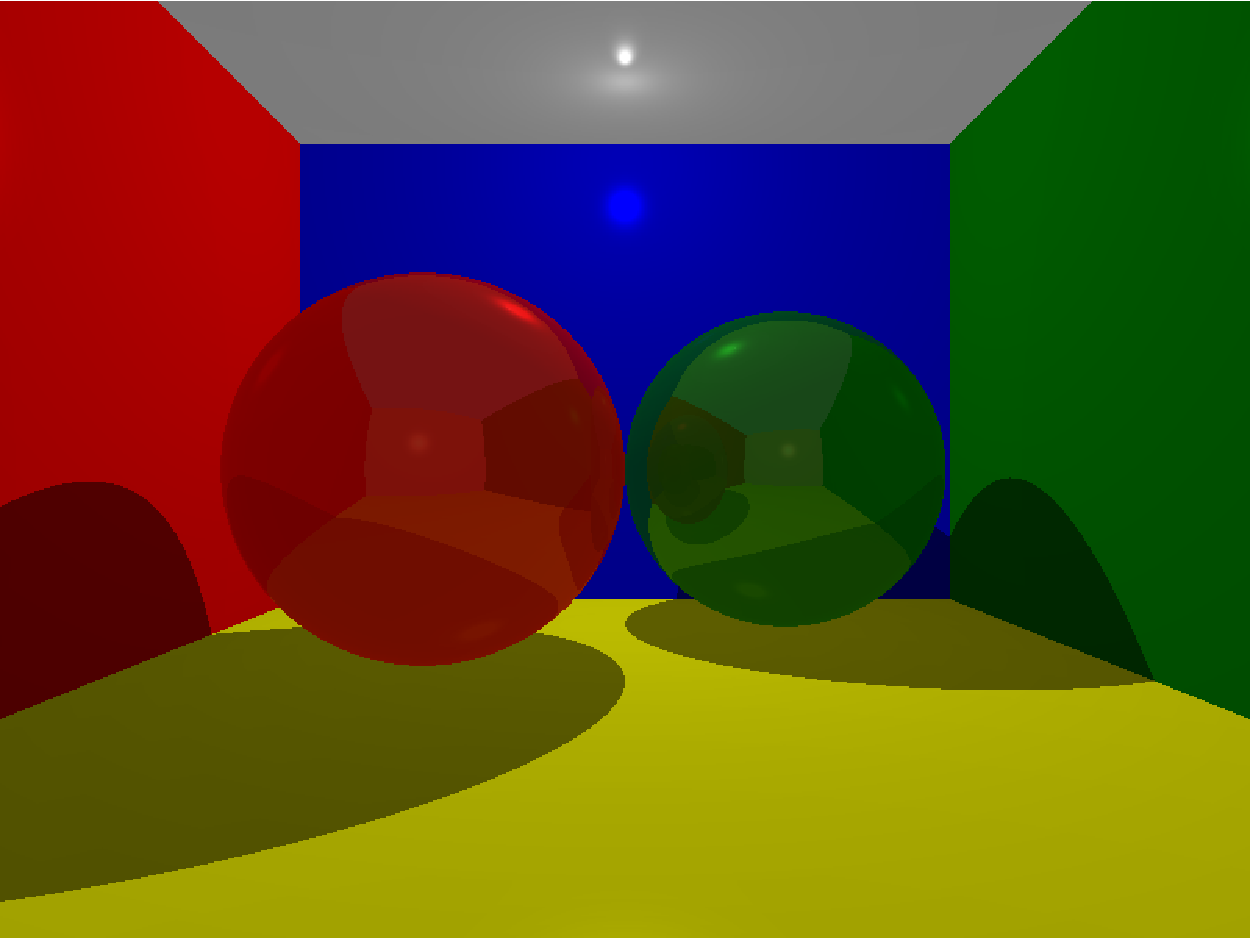
\includegraphics[width=0.55\textwidth]{test14}
	\caption{Визуализация функционального теста №14}
	\label{fig:test14}
\end{figure}

\section{Модульное тестирование}
Модульное тестирование было реализовано с помощью фреймворка XUnit~\cite{XUnit}. В качестве метрики, используемой для оценки полноты тестирования программного обеспечения, было выбрано покрытие строк кода. Реализованный набор модульных тестов имеет покрытие, равное 23\%.

Примеры модульных тестов приведены на листингах~\ref{lst:VAdd}~-~\ref{lst:HSphere}.
\clearpage
\begin{center}
	\begin{lstlisting}[linewidth=\linewidth, label={lst:VAdd}, captionpos={t}, caption={Пример модульного теста для сложения двух векторов}]
	[Fact]
	public void AdditionOperatorTest()
	{
		var v1 = new Vector3(1, 2, 3);
		var v2 = new Vector3(4, 5, 6);
		var result = v1 + v2;
		
		Assert.True(result.X == 5 && result.Y == 7 && result.Z == 9);
	}
	\end{lstlisting}
\end{center}

\begin{center}
	\begin{lstlisting}[linewidth=\linewidth, label={lst:HSphere}, captionpos={t}, caption={Пример модульного теста для неуспешного поиска пересечения луча со сферой}]
	[Fact]
	public void SphereIntersectRay_MissesSphere()
	{
		var sphere = new Sphere(new Vector3(0, 0, -5), 1, System.Drawing.Color.Red, 0);
		var ray = new Ray(new Vector3(0, 0, 0), new Vector3(1, 0, 0));
		
		bool hit = sphere.IntersectRay(ray, out double distance, out Vector3 normal);
		
		Assert.False(hit);
	}
	\end{lstlisting}
\end{center}

\clearpage
\section{Интерфейс программного обеспечения}
На рисунке~\ref{fig:InterfaceDemoStart} приведена демонстрация интерфейса программы при ее запуске.
\begin{figure}[H]
	\centering
	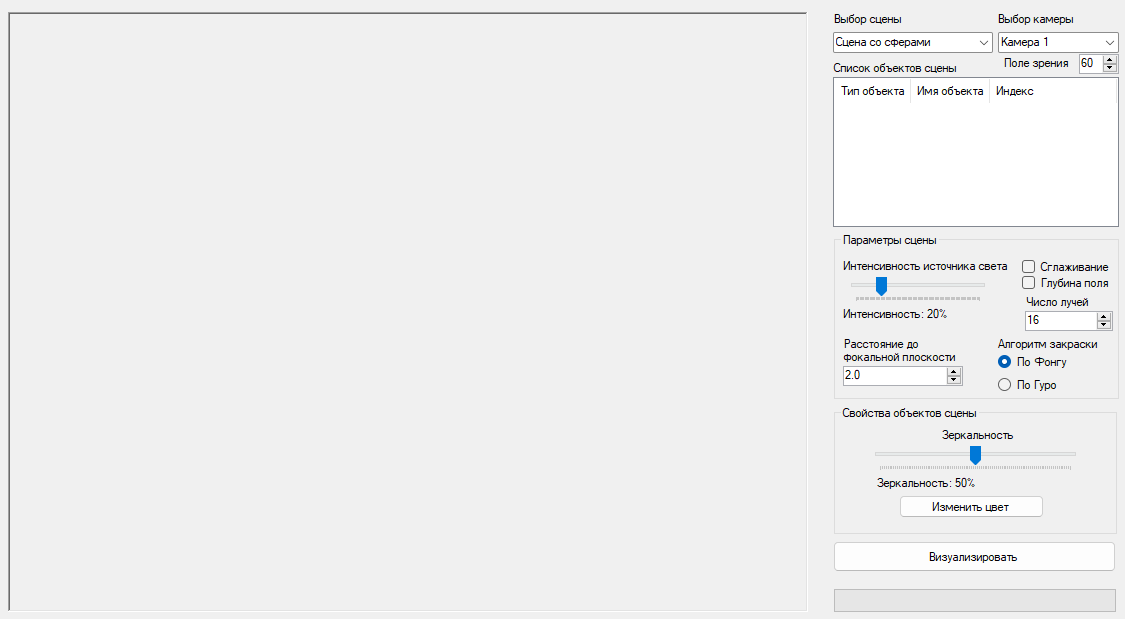
\includegraphics[width=0.8\textwidth]{InterfaceDemoStart}
	\caption{Пользовательский интерфейс ПО}
	\label{fig:InterfaceDemoStart}
\end{figure}

В левой части окна приложения расположена графическая область в виде прямоугольника для отображения результатов визуализации. На любой объект сцены можно произвести нажатие левой кнопки мыши, после чего выбранный объект будет выделен в окне <<Список объектов сцены>> и объект будет доступен для изменения параметров.

Пользователю на выбор предоставляются три варианта сцены, на каждом из них возможен выбор трех вариантов расположения камер. Изменяемым параметром камеры является ее поле зрения. Пример выбора сцены и камеры приведен на рисунке~\ref{fig:ChoosingSceneDemo}.

Ниже перечисленных элементов графического интерфейса расположено окно <<Список объектов сцены>>, который заполняется наименованиями объектов сцены при нажатии кнопки <<Визуализировать>>. В данном элементе можно выбирать объекты сцены нажатием левой кнопки мыши на нужную строку для изменения свойств выбранного объекта.

Группа параметров <<Параметры сцены>> позволяет настроить общие для всех объектов параметры. Пользователю предоставлена возможность изменить интенсивность источника света, включить сглаживание (Anti-Aliasing)~\cite{Anti-aliasing} и глубину поля, выбрать число лучей для двух описанных эффектов, изменить расстояние от камеры до фокальной точки (расстояние измеряется по вектору направлению взгляда), а также выбрать алгоритм закраски -- по методу Фонга или по методу Гуро.

Группа параметров <<Свойства объектов сцены>> позволяет настроить зеркальность поверхности выбранного объекта и его цвет. Пример выбора объекта сцены и изменения его зеркальности приведен на рисунке~\ref{fig:ChoosingObjectDemo}.

Для вступления в силу любого из перечисленных изменений параметров необходимо нажать кнопку <<Визуализировать>>, после чего дождаться визуализации сцены (под кнопкой расположена полоса статуса для отображения прогресса визуализации).

\begin{figure}[H]
	\centering
	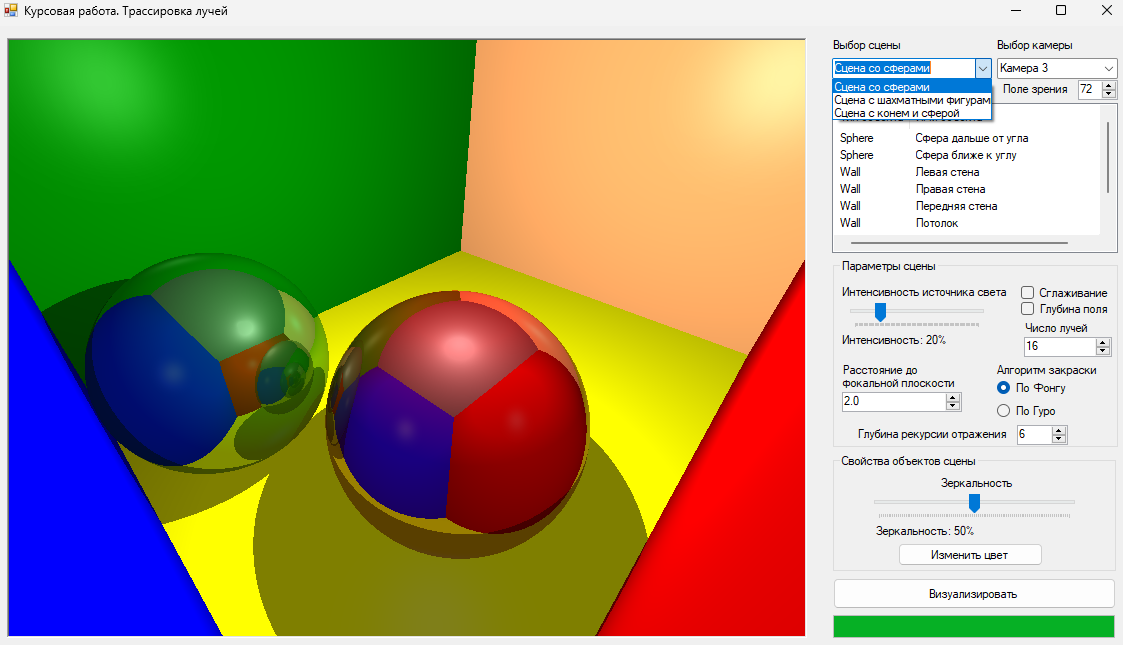
\includegraphics[width=0.8\textwidth]{ChoosingSceneDemo}
	\caption{Пример выбора сцены и камеры}
	\label{fig:ChoosingSceneDemo}
\end{figure}

\begin{figure}[H]
	\centering
	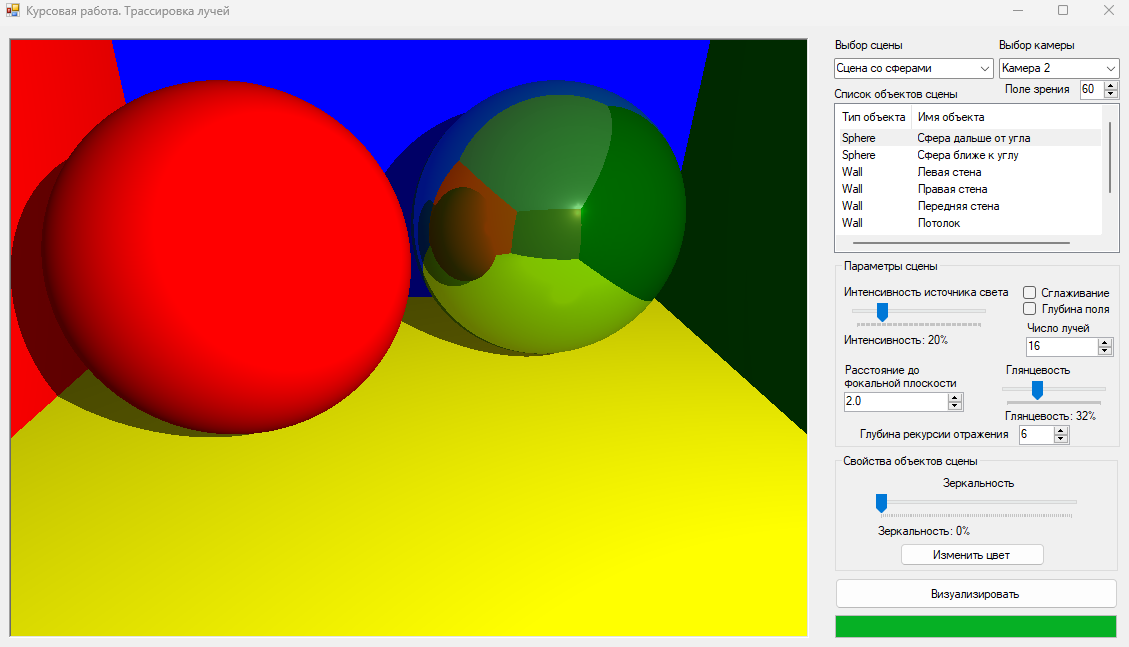
\includegraphics[width=0.8\textwidth]{ChoosingObjectDemo}
	\caption{Пример выбора объекта на сцене и изменения его зеркальности}
	\label{fig:ChoosingObjectDemo}
\end{figure}

\section*{Вывод}
В данном разделе были выбраны средства реализации, описана структура классов программы и ее тестирование, а также приведено описание интерфейса ПО.

\clearpage
